\chapter{\textcolor{purple}{Chapitre 2 : Spécification des besoins & Réalisation}}
\section{\textcolor{cyan}{Spécification des besoins:}}
\subsection{Besoin spécifié:}
Dans le domaine de web la communication entre les utilisateurs devient une nécessité, et le communication vidéo et audio a une interactivité mieux que les messages, donc Djagora veut une plateforme de communication sécurisé qui permet à ses employées de se connecter dans un space privé sans utiliser les plateformes comme Google meet ou discord et mettre des réunions dans des room de chat.\par
Lorsque l’utilisateur fait un login il peut joindre un room qui est identifié par un code, ce code est nécessaire pour entrer ou sortir de room.\par
Ce plateforme est un plateforme web, notre tâche se présente dans l’authentication le développement de login et sign up avec le chat vidéo ou audio seulement.\par
Dans ce cas, on a utilisé l’API de WEBRTC qui va assurer la communication entre les différents employées de la même room.\par
\subsection{Webrtc:}
C’est quoi webrtc?\newline
Il permet d’ajouter des capacités de communication en temps réel à l’application qui fonctionne sur la base d'une norme ouverte. Elle prend en charge la vidéo, la voix et les données génériques à envoyer entre pairs, ce qui permet aux développeurs de créer de puissantes solutions de communication vocale et vidéo.\par
La technologie est disponible sur tous les navigateurs modernes ainsi que sur des clients natifs pour toutes les principales plateformes. Les technologies qui sous-tendent le Webrtc sont mises en œuvre en tant que norme Web ouverte et disponibles sous forme d'API JavaScript ordinaires dans tous les principaux navigateurs. Pour les clients natifs, comme les applications Android et iOS, il existe une bibliothèque qui offre la même fonctionnalité. Le projet Webrtc est open-source et soutenu par Apple, Google, Microsoft et Mozilla, entre autres.\par
\section{\textcolor{cyan}{Réalisation :}}
\subsection{\textcolor{cyan}{Les technologies utilisées : Node.js et express:}}
\begin{enumerate}[label=(\alph*)]
    \item \textbf{node:}\\
    Node (ou plus formellement Node.js) est un environnement d'exécution open-source et multiplateforme qui permet aux développeurs de créer toutes sortes d'outils et d'applications côté serveur en JavaScript. Le moteur d'exécution est destiné à être utilisé en dehors du contexte d'un navigateur (c'est-à-dire en s'exécutant directement sur un ordinateur ou un système d'exploitation serveur). En tant que tel, l'environnement omet les API JavaScript spécifiques au navigateur et ajoute la prise en charge d'API de système d'exploitation plus traditionnelles, notamment HTTP et les bibliothèques de système de fichiers.\par
Du point de vue du développement d'un serveur web, Node présente un certain nombre d'avantages :\par
\begin{itemize}
    \item Excellentes performances ! Node a été conçu pour optimiser le débit et l'évolutivité des applications Web et constitue une bonne solution pour de nombreux problèmes courants de développement Web (par exemple, les applications Web en temps réel).\par
    \item Le code est écrit en "plain old JavaScript", ce qui signifie que moins de temps est passé à gérer le "changement de contexte" entre les langages lorsque vous écrivez du code côté client et côté serveur.\par
    \item JavaScript est un langage de programmation relativement nouveau et bénéficie d'améliorations dans la conception du langage par rapport à d'autres langages traditionnels de serveur Web (par exemple, Python, PHP, etc.). De nombreux autres langages nouveaux et populaires se compilent/se convertissent en JavaScript, de sorte que vous pouvez également utiliser TypeScript, CoffeeScript, ClojureScript, Scala, LiveScript, etc.\par
    \item Le gestionnaire de paquets node (NPM) donne accès à des centaines de milliers de paquets réutilisables. Il dispose également de la meilleure résolution de dépendances de sa catégorie et peut être utilisé pour automatiser la majeure partie de la chaîne d'outils de construction.\par
    \item Node.js est portable. Il est disponible sur Microsoft Windows, macOS, Linux, Solaris, FreeBSD, OpenBSD, WebOS et NonStop OS. En outre, il est bien supporté par de nombreux fournisseurs d'hébergement web, qui fournissent souvent une infrastructure et une documentation spécifiques pour l'hébergement de sites Node.\par
\end{itemize}
\item \textbf{Express:}\\
Express est le Framework web Node le plus populaire, et est la bibliothèque sous-jacente pour un certain nombre d'autres Framework web Node populaires. Il fournit des mécanismes pour :\par
\begin{itemize}
    \item Écrire des gestionnaires pour les demandes avec différents requêtes HTTP à différents chemins URL (routes).
    \item Intégrer des moteurs de rendu de type "vue" afin de générer des réponses en insérant des données dans des modèles.\par
    \item Définissez les paramètres courants des applications Web, comme le port à utiliser pour la connexion et l'emplacement des modèles utilisés pour le rendu de la réponse.\par
    \item Ajouter un middleware supplémentaire de traitement des demandes à n'importe quel point du pipeline de traitement des demandes.
\end{itemize}
Bien qu'Express soit en soi assez minimaliste, les développeurs ont créé des paquets de middleware compatibles pour répondre à presque tous les problèmes de développement Web. \par
Il existe des bibliothèques 	permettant de travailler avec les cookies, les sessions, les connexions 	d'utilisateurs, les paramètres d'URL, les données POST, les en-têtes de sécurité, et bien d'autres encore. Vous trouverez une liste des paquets de middleware maintenus par l'équipe Express à l'adresse Express 	Middleware (ainsi qu'une liste de certains paquets tiers populaires).\par
\end{enumerate}
\subsection{\textcolor{cyan}{Les interfaces}}
    \centering
    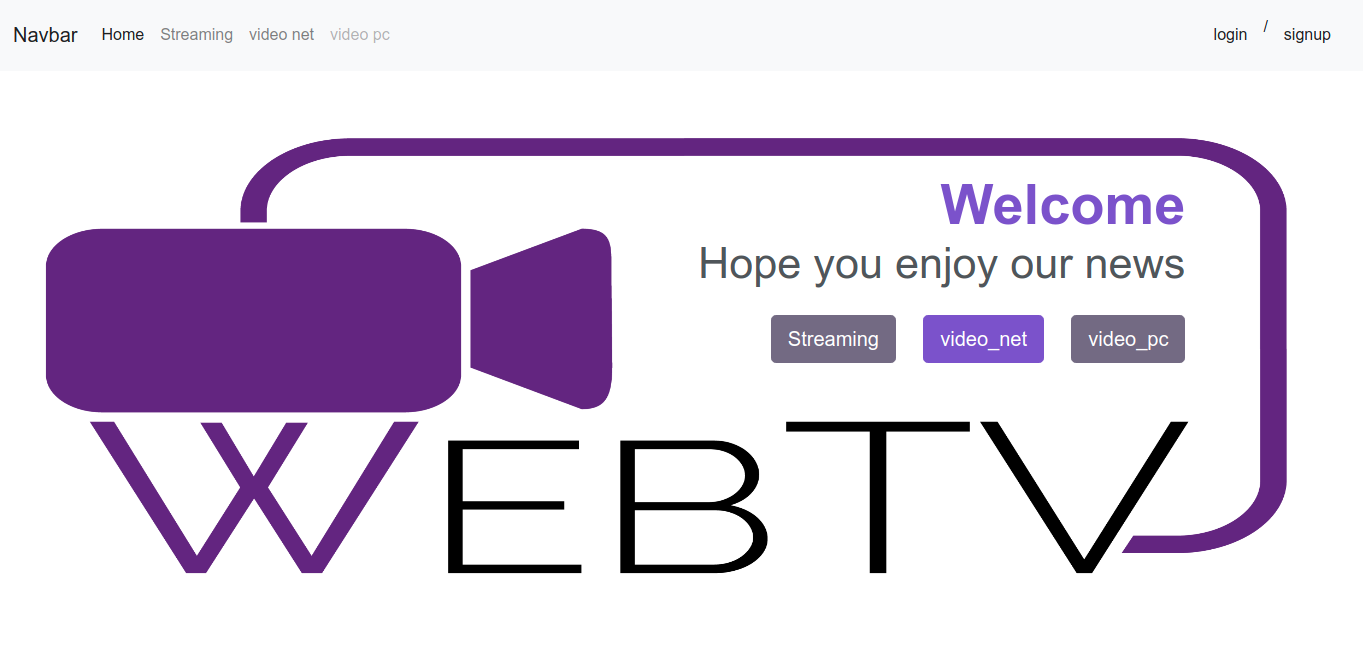
\includegraphics[width=12cm]{images/indexPage.png}\\
C’est la page d’accueil de notre application, il y a 3 boutons chacun d’entre eux comporte comme un lien.\par
    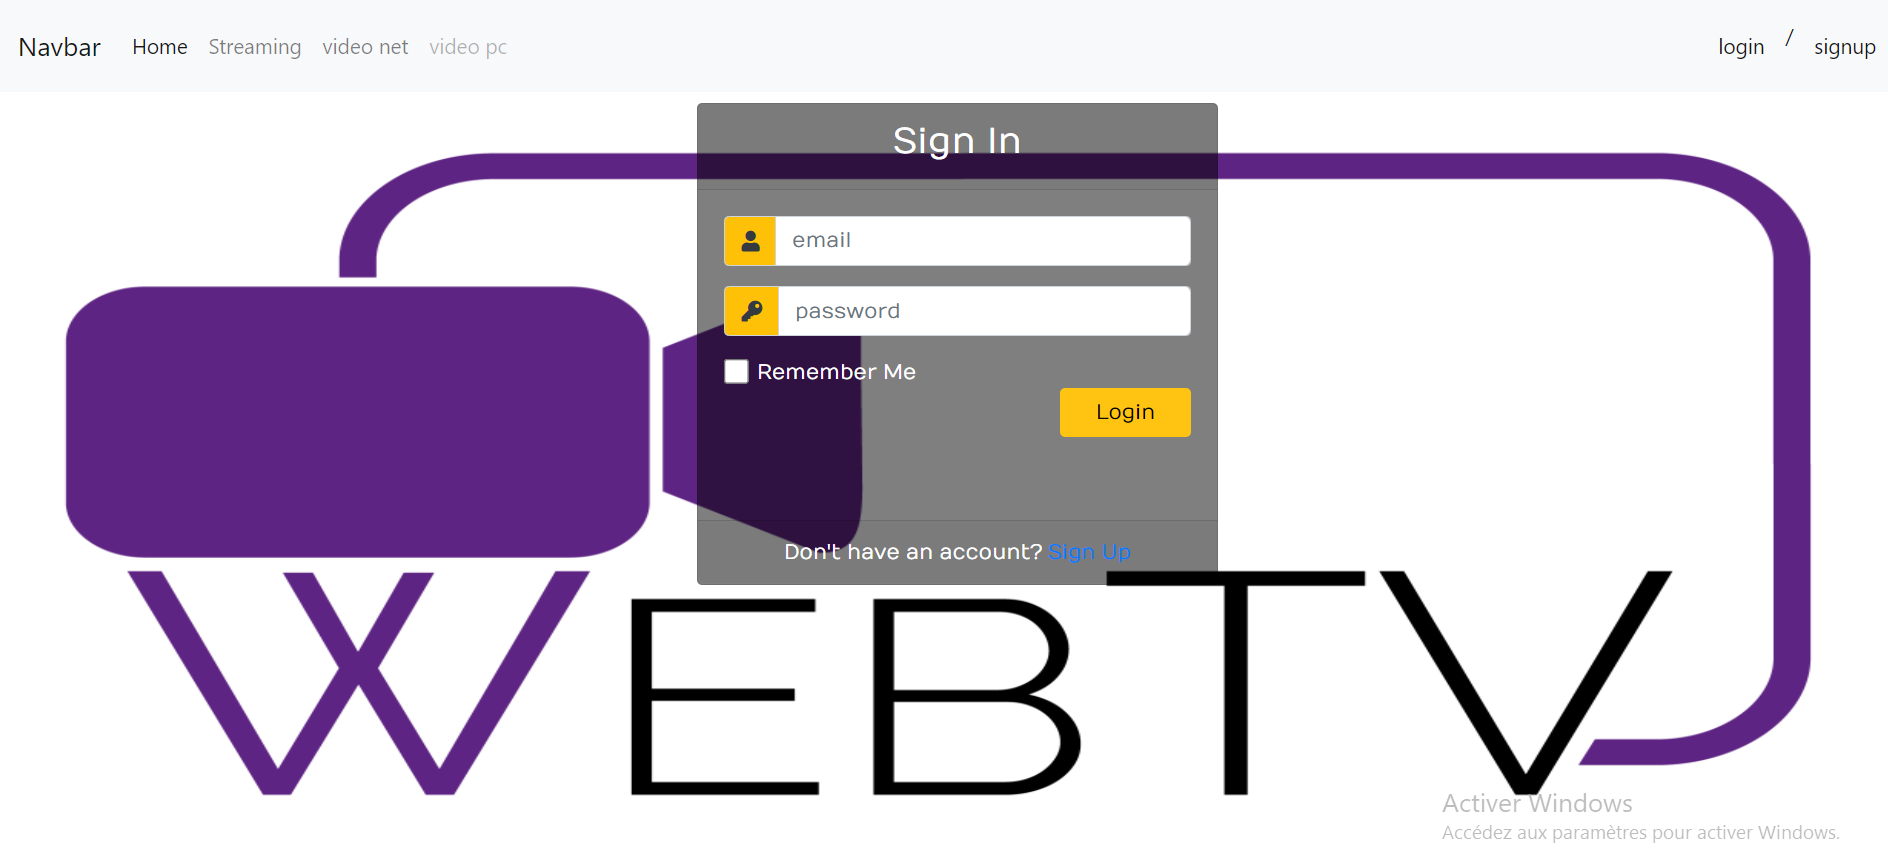
\includegraphics[width=12cm]{images/authentificationPage.png}\\
    C’est la page d’authentification des utilisateurs en entrant l’ email et le mots de passe pour ouvrir une session.\par
    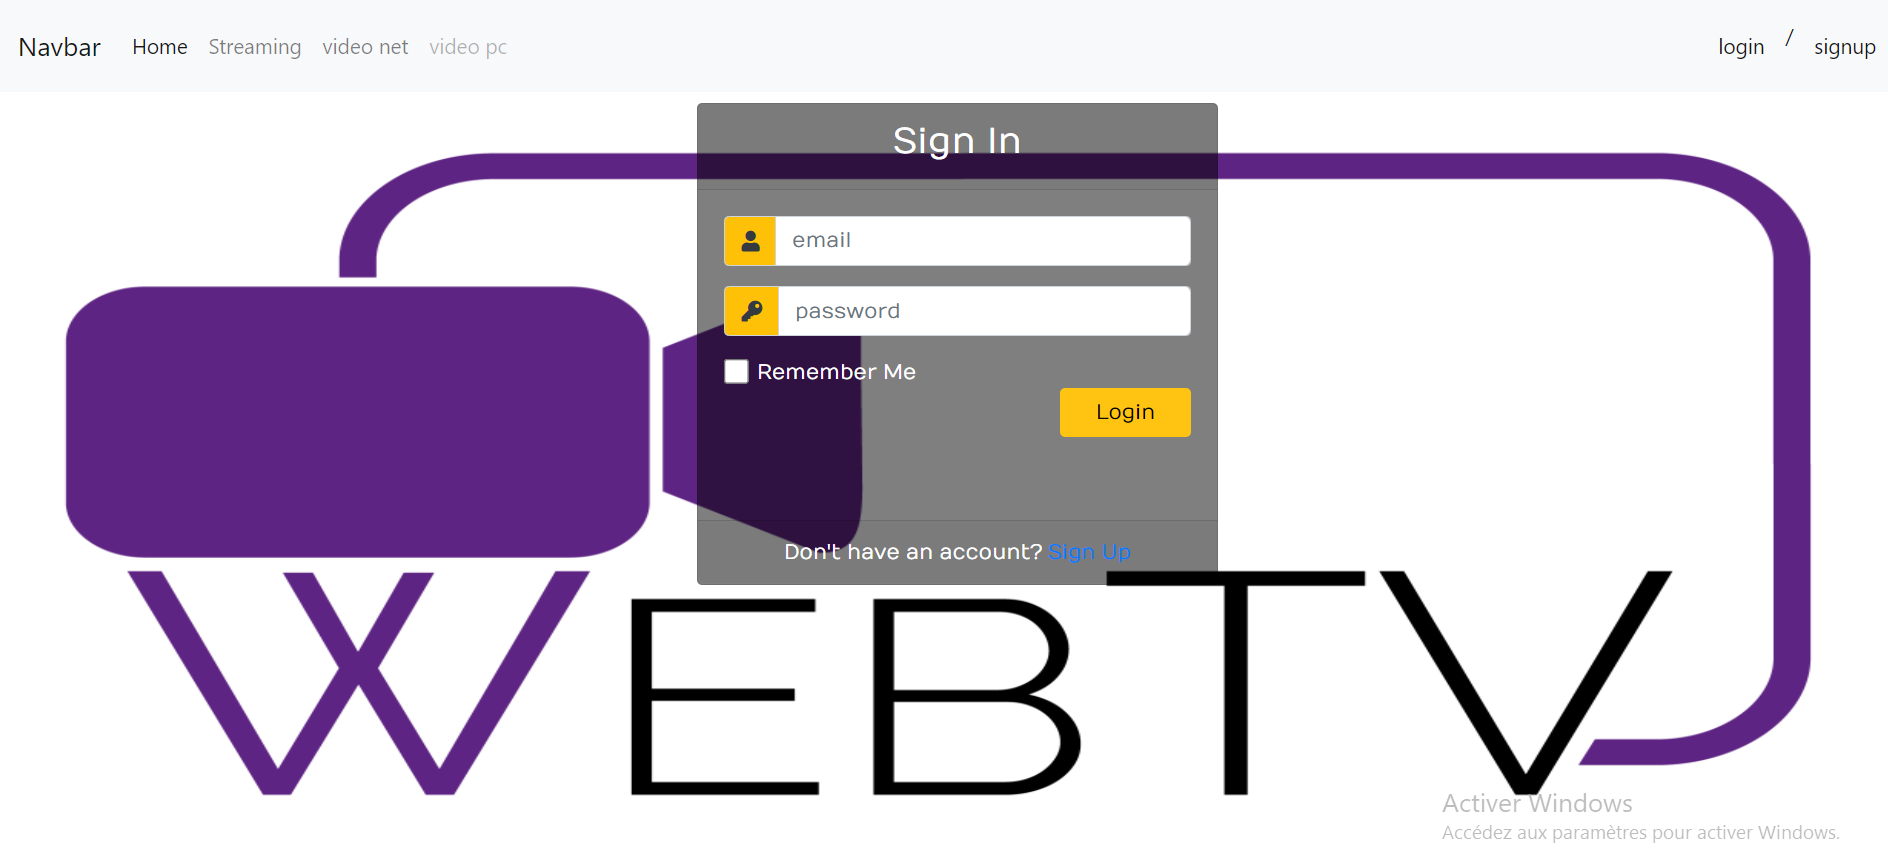
\includegraphics[width=12cm]{images/authentificationPage.png}\\
    En cliquant sur le bouton «video net », un vidéo va s’ouvrit sur la page.\par
    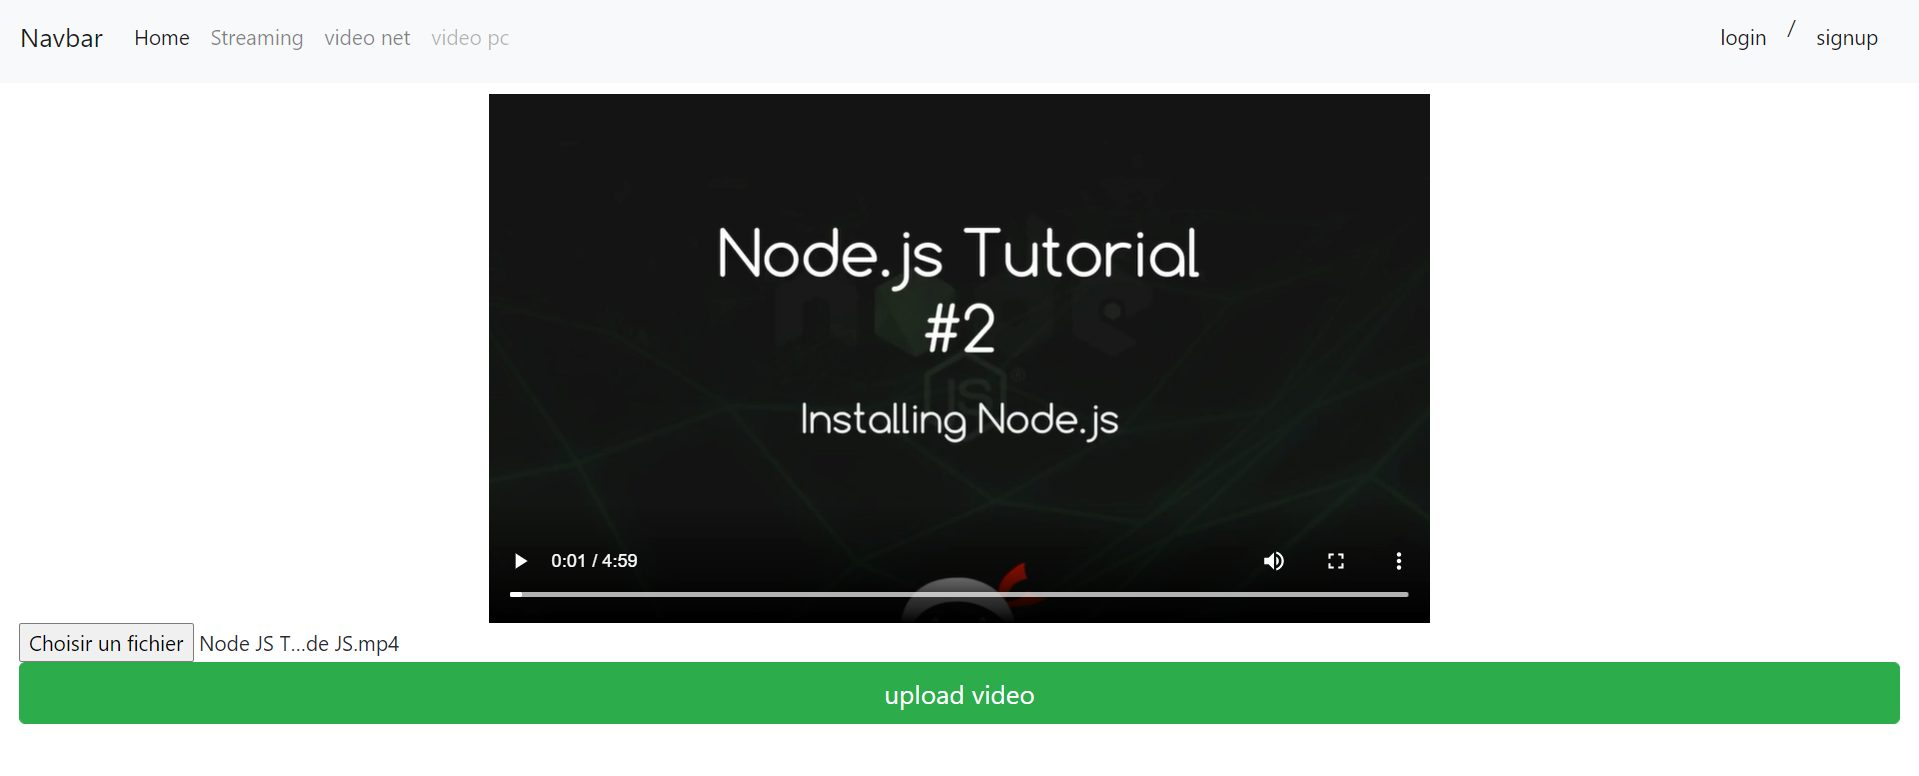
\includegraphics[width=15cm]{images/videoPc2.png}\\
    En cliquant sur le bouton « Choisir un fichier » , un dialogue s’ouvrit qui n’accepte que les fichiers vidéo et en choisissant un vidéo enregistré dans le pc, la page va s’ouvrit le vidéo choisi.\par
    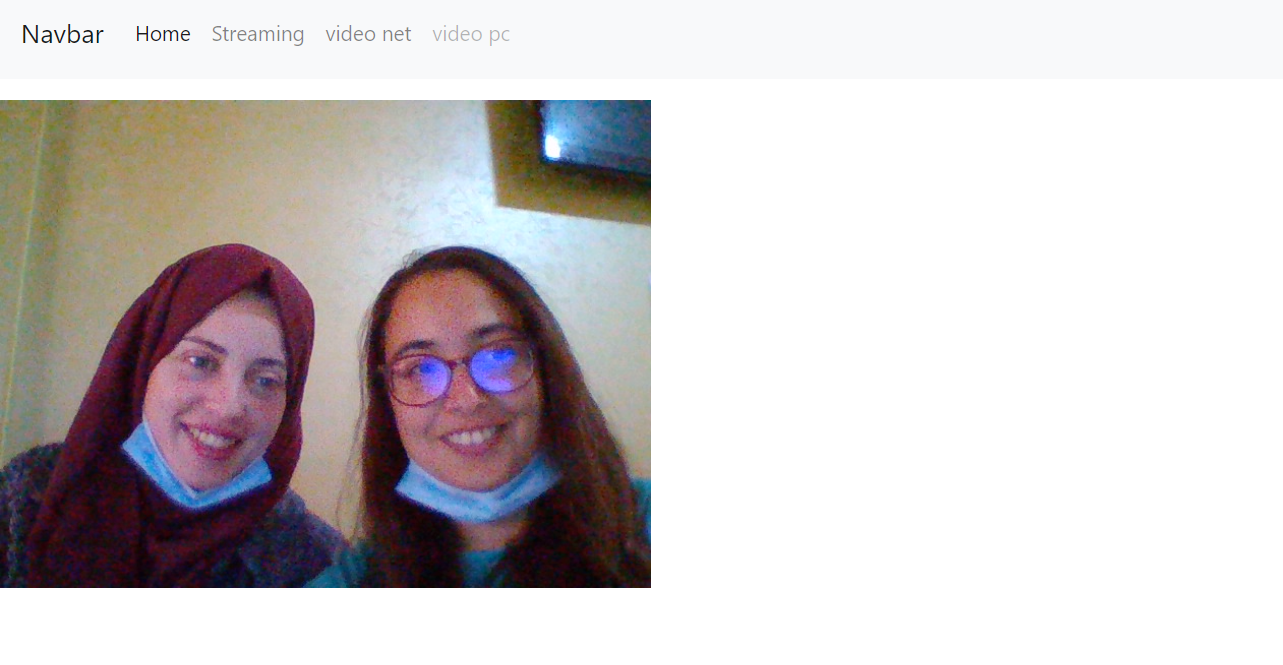
\includegraphics[width=15cm]{images/streaming.png}\\
    En cliquant sur le bouton « Streaming », cette page va s’ouvrit contenant une demande d’ouvrir le Cam et l’audio. En acceptant une entre eux, l’utilisateur va joindre le room .\par

\subsection{\textcolor{cyan}{deploiement heroku}}
Heroku est un PaaS (Platform as a Service) destinée au développement dans le Cloud. Heroku prend en charge les langages Ruby on Rails, Java, JavaScript, Node.js, Python, Scala et Clojure.\par
\subsection{\textcolor{cyan}{lien du travail}}
\hyperlink{https://webapprtcsahareya.herokuapp.com/}{\textcolor{red}{https://webapprtcsahareya.herokuapp.com/}}\\

\includegraphics[width=15cm]{images/heroku.png}\\